\documentclass[10pt]{beamer}

\usepackage[utf8]{inputenc}
\usepackage[polish]{babel}
\usepackage[T1]{fontenc}
\usepackage{graphicx}
\usepackage{animate}
\usepackage{hyperref}

\hypersetup{
    colorlinks=true,
    linkcolor=[RGB]{214, 2, 73},
    filecolor=magenta,
    urlcolor=[RGB]{173, 2, 230},
    pdftitle={prez},
    pdfpagemode=FullScreen,
}

\usetheme{Warsaw}
\usecolortheme{albatross}

\title{Inercyjne utrzymywanie plazmy}
\subtitle{}
\author{Maciej Jerzyk, Mikołaj Krenc}
\date{21.01.2025r.}

\begin{document}

    \begin{frame}
        \titlepage{}
    \end{frame}

    \begin{frame}{Spis Treści}
        \tableofcontents
    \end{frame}

    \section{Wprowadzenie}

        \begin{frame}{Co to jest plazma?}
            \begin{itemize}
                \item \textbf{Plazma} - jedna z czterech podstawowych stanów materii charakteryzująca się dużą koncentracją jonów.
                \item Jednym ze sposobów otrzymywania plazmy jest podgrzanie materii do wysokiej temperatury, mowa tu o temperaturach sięgających 10000\ K. Energia elektronu w plazmie o wysokiej temperaturze może wynosić aż 100\ eV!
                \item Inne techniki otrzymywania plazmy wykorzystują pole magnetyczne.
            \end{itemize}

            \raggedright{}
            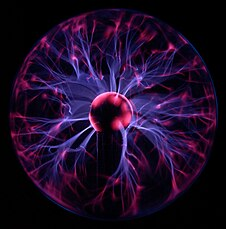
\includegraphics[width=0.4\textwidth]{lamp.jpg}

        \end{frame}

        \begin{frame}{Plazma powstająca w naturze nierzadko osiąga takie, i dużo wyższe parametry.}
            \begin{minipage}{0.49\textwidth}
                \centering
                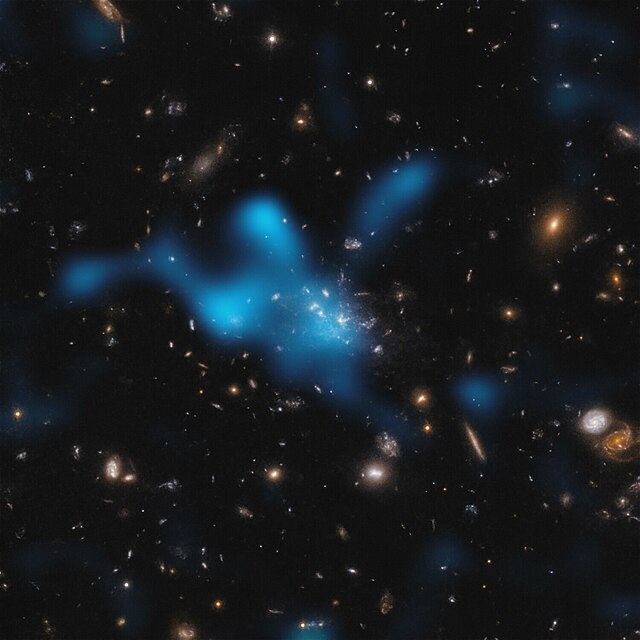
\includegraphics[width=0.8\linewidth]{intracluster.jpg}
            \end{minipage}
            \hfill
            \begin{minipage}{0.49\textwidth}
                \centering
                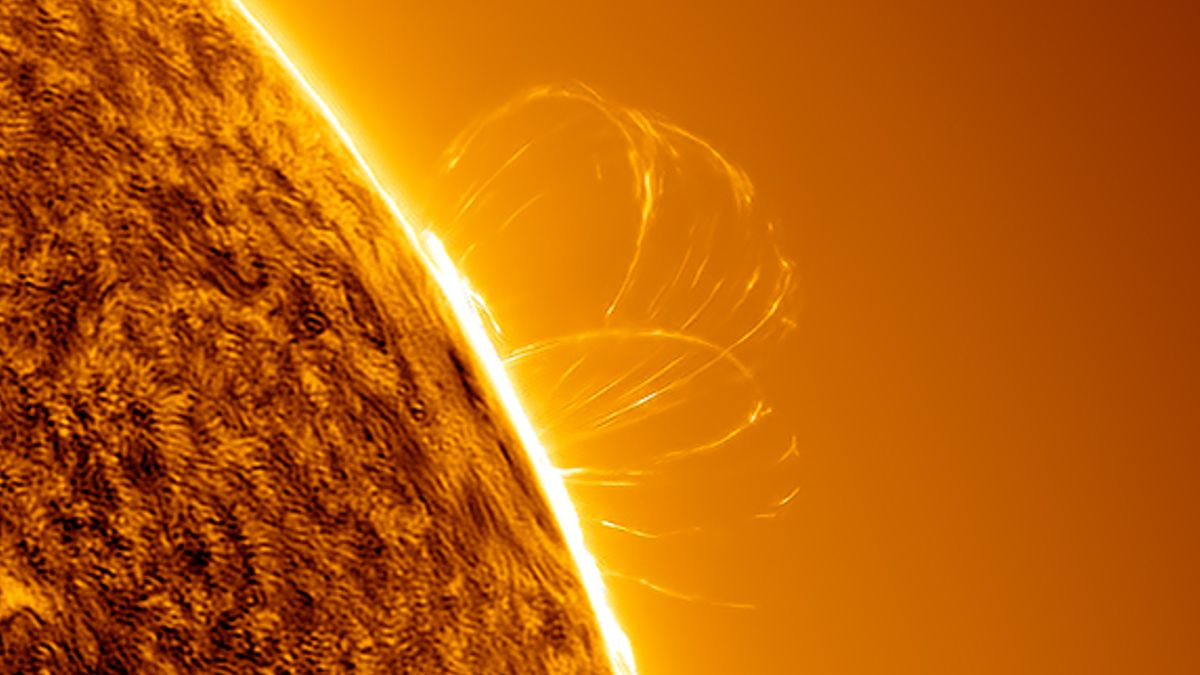
\includegraphics[width=0.8\linewidth]{star.jpg}
            \end{minipage}
        \end{frame}

        \begin{frame}{Ale my musimy się jeszcze wiele nauczyć\dots}
            \begin{minipage}{0.49\textwidth}
                \centering
                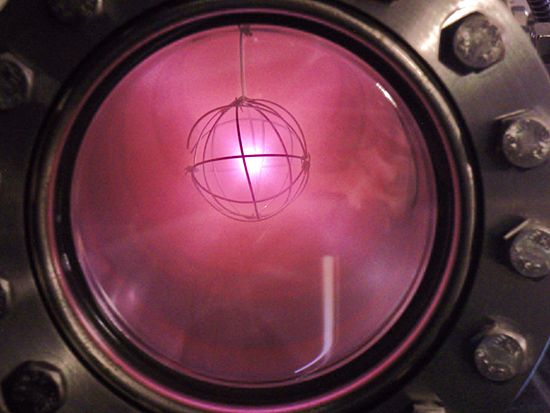
\includegraphics[width=0.8\linewidth]{deuterium.jpg}
            \end{minipage}
            \hfill
            \begin{minipage}{0.49\textwidth}
                \centering
                
\includegraphics[width=0.8\linewidth]{patrick.jpeg}
            \end{minipage}
        \end{frame}

    \section{Metody sztucznego otrzymywania plazmy}

    \begin{frame}{Wybrane metody sztucznego otrzymywania plazmy}
        \begin{minipage}{0.49\textwidth}
            \centering
            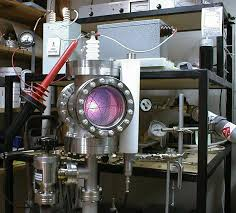
\includegraphics[width=0.8\linewidth]{fusor.jpg}
        \end{minipage}
        \hfill
        \begin{minipage}{0.49\textwidth}
            \centering
            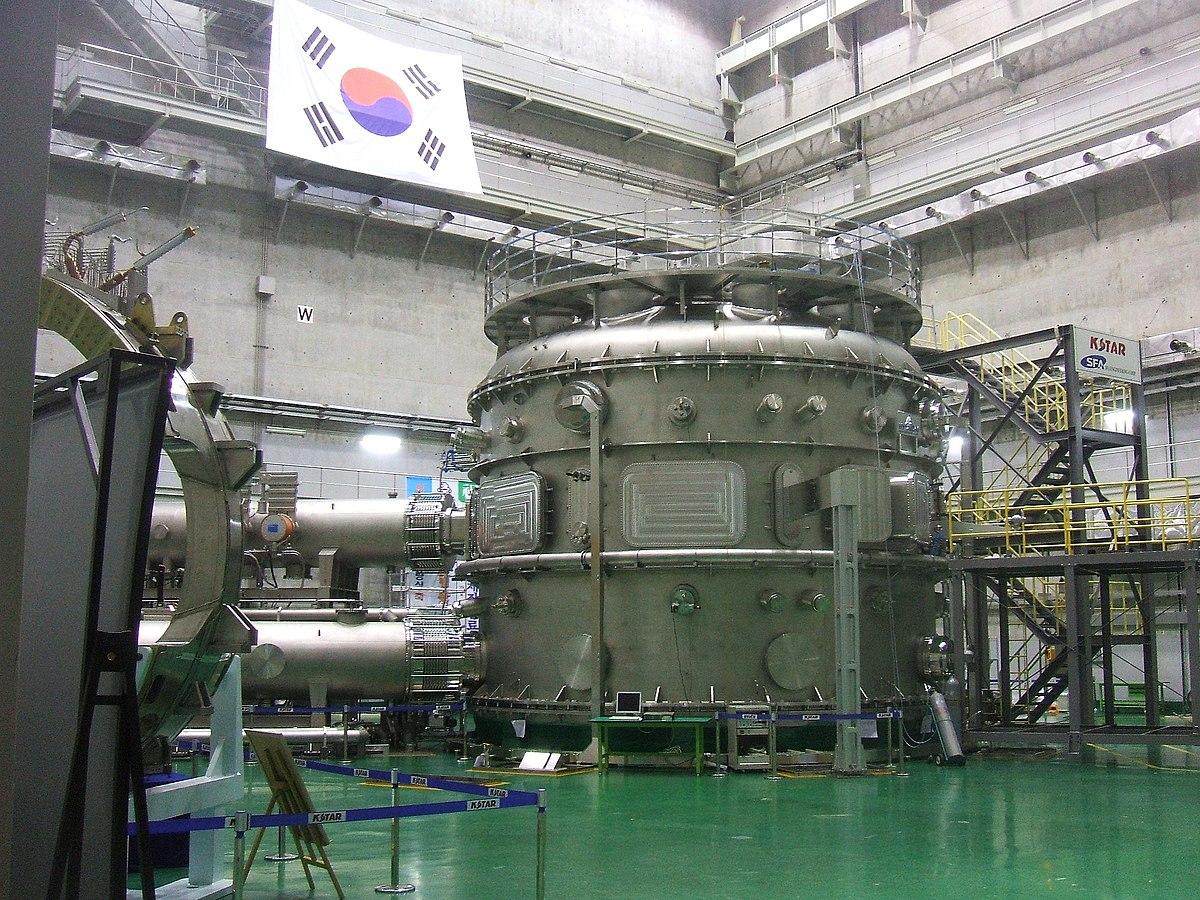
\includegraphics[width=0.8\linewidth]{tokamak.jpeg}
        \end{minipage}
    \end{frame}


\end{document}
